\documentclass[aspectratio=169]{beamer}

\usetheme{Madrid}
\usecolortheme{whale}
\usepackage[utf8]{inputenc}
\usepackage{booktabs}
\usepackage{tikz}
\usetikzlibrary{arrows.meta, positioning, fit, backgrounds}

\setbeamertemplate{navigation symbols}{}
\setbeamertemplate{footline}[frame number]
\setbeamercolor{block title}{bg=blue!20,fg=black}
\setbeamercolor{block body}{bg=blue!5,fg=black}
\setbeamercolor{alertblock title}{bg=red!20,fg=black}
\setbeamercolor{alertblock body}{bg=red!5,fg=black}
\setbeamercolor{exampleblock title}{bg=green!25,fg=black}
\setbeamercolor{exampleblock body}{bg=green!8,fg=black}

\title[BDH-Swapped AttnGrounder]{Swapping AttnGrounder's Attention for a\\ Brain-Inspired Associative Memory (BDH)}
\subtitle{Testing the ``Grounding = In-Context Retrieval'' Hypothesis on Talk2Car}
\author{Sudarshan Sudhakar}
\date{\today}

\begin{document}

% ------------------------------------------------------------------
\begin{frame}
  \titlepage
\end{frame}

% ------------------------------------------------------------------
\begin{frame}{Outline}
  \tableofcontents
\end{frame}

\section{Motivation \& Hypothesis}

% ------------------------------------------------------------------
\begin{frame}{The Task: Visual Grounding}
  \begin{columns}[T]
    \begin{column}{0.55\textwidth}
      \textbf{Visual grounding} (Talk2Car): given an image and a
      natural-language command, localize the single object the
      command refers to.
      \vspace{0.4cm}

      \textit{``Turn left behind the silver car''} $\rightarrow$
      one bounding box.

      \vspace{0.4cm}
      The hard cases are scenes with \textbf{multiple objects of the
      same class} — the model must disambiguate using language, not
      just detect.
    \end{column}
    \begin{column}{0.45\textwidth}
      \begin{block}{Baseline model}
        \textbf{AttnGrounder} (Mittal, IIT Mandi) — single-stage,
        Darknet-53 + BiLSTM/GloVe, a lightweight \emph{visual--text
        attention} module fuses the two modalities before a YOLO head.
      \end{block}
    \end{column}
  \end{columns}
\end{frame}

% ------------------------------------------------------------------
\begin{frame}{Why Bring in BDH?}
  \begin{block}{Dragon Hatchling (BDH) — Kosowski et al., Pathway 2025}
    A brain-inspired sequence architecture whose working memory is an
    \textbf{explicit, growing outer-product associative memory}
    ($\rho = K^\top V$), updated with Hebbian-style read/write —
    rather than a fixed-size compressed state (e.g.\ Mamba/SSMs).
  \end{block}
  \vspace{0.3cm}
  \begin{alertblock}{The hypothesis we're testing}
    \emph{``Grounding = in-context retrieval''}: architectures with
    explicit associative memory should have an edge precisely when a
    query must be matched against \textbf{multiple similar
    candidates} in context — because that is a retrieval problem, not
    a compression problem.
  \end{alertblock}
  \textbf{Prediction:} swapping AttnGrounder's attention for a BDH
  module should raise AP50 \emph{disproportionately} on scenes with
  several same-class candidate objects (``ambiguous'' scenes),
  relative to scenes with only one.
\end{frame}

\section{Method}

% ------------------------------------------------------------------
\begin{frame}{Architecture: A Drop-In Swap}
  \begin{center}
  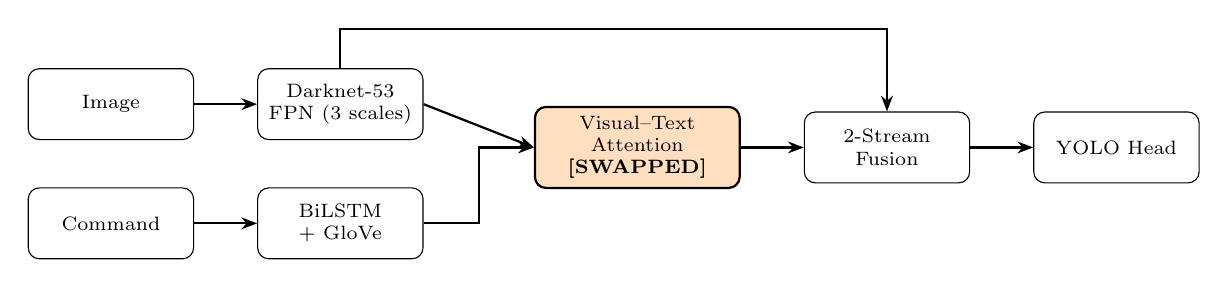
\begin{tikzpicture}[
      node distance=6mm and 8mm,
      box/.style={draw, rounded corners, minimum height=0.9cm, minimum width=2.1cm, align=center, font=\scriptsize},
      swap/.style={draw, rounded corners, minimum height=0.9cm, minimum width=2.6cm, align=center, font=\scriptsize, fill=orange!25, thick},
      arrow/.style={-{Stealth[length=2mm]}, thick}
  ]
    \node[box] (img) {Image};
    \node[box, below=of img] (txt) {Command};

    \node[box, right=of img] (visu) {Darknet-53\\FPN (3 scales)};
    \node[box, right=of txt] (lang) {BiLSTM\\+ GloVe};

    \node[swap, right=14mm of visu, yshift=-0.55cm] (attn) {Visual--Text\\Attention\\\textbf{[SWAPPED]}};

    \node[box, right=of attn] (fuse) {2-Stream\\Fusion};
    \node[box, right=of fuse] (yolo) {YOLO Head};

    \draw[arrow] (img) -- (visu);
    \draw[arrow] (txt) -- (lang);
    \draw[arrow] (visu.east) -- (attn.west);
    \draw[arrow] (lang.east) -- ++(0.7,0) |- (attn.west);
    \draw[arrow] (attn) -- (fuse);
    \draw[arrow] (visu.north) -- ++(0,0.5) -| (fuse.north);
    \draw[arrow] (fuse) -- (yolo);
  \end{tikzpicture}
  \end{center}
  \vspace{0.2cm}
  \begin{columns}[T]
    \begin{column}{0.48\textwidth}
      \small\textbf{Baseline attention:} softmax cross-attention
      (region queries $\times$ word keys), scalar gate $\beta$.
    \end{column}
    \begin{column}{0.48\textwidth}
      \small\textbf{BDH module:} symmetric or causal-context kernel
      (3 modes tried, see Results); ReLU-sparse addressing; explicit
      outer-product memory; multiplicative bilinear gate. Same output
      shapes $\Rightarrow$ true drop-in.
    \end{column}
  \end{columns}
\end{frame}

% ------------------------------------------------------------------
\begin{frame}{Keeping the Comparison Fair}
  \begin{itemize}
    \item \textbf{Single component swap}: backbone, text encoder, YOLO
      head, losses, hyperparameters — all byte-for-byte identical
      between variants.
    \item \textbf{Fusion trim}: BDH fuses only $[f_{visu}, f_{lang\_attn}]$
      (2 streams) instead of the original 3, to offset most of the
      module's added parameters.
    \item \textbf{Same training recipe for all variants}: A100-40GB,
      bf16, 100 epochs, Adam (lr $10^{-4}$, backbone lr$/10$), batch
      14, poly LR schedule.
  \end{itemize}
  \vspace{0.3cm}
  \begin{table}
    \centering\small
    \begin{tabular}{lccc}
      \toprule
      Variant & Params & vs.\ baseline \\
      \midrule
      Baseline (AttnGrounder, unmodified) & 75.84M & --- \\
      BDH (any mode, single-head) & 76.63M & $+0.79$M ($+1.0\%$) \\
      \bottomrule
    \end{tabular}
  \end{table}
  \small Backbone dominates parameter count either way — this is a
  fusion-mechanism comparison, not a capacity comparison.
\end{frame}

\section{How We Measure Success}

% ------------------------------------------------------------------
\begin{frame}{The Metrics, Explained}
  \begin{columns}[T]
    \begin{column}{0.5\textwidth}
      \begin{block}{AP50 (our headline number)}
        \small A prediction counts as \textbf{correct} if the
        predicted box overlaps the ground-truth box by
        \textbf{Intersection-over-Union} $\geq 0.5$. AP50 = \% of
        commands localized correctly.
      \end{block}
      \begin{center}
      \scalebox{0.55}{
      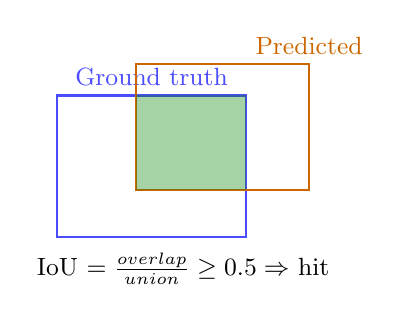
\begin{tikzpicture}[every node/.style={font=\small}]
        \draw[thick, blue!70] (0,0) rectangle (2.4,1.8);
        \node[blue!70, above] at (1.2,1.8) {Ground truth};
        \draw[thick, orange!80!black] (1.0,0.6) rectangle (3.2,2.2);
        \node[orange!80!black, above] at (3.2,2.2) {Predicted};
        \begin{scope}
          \clip (0,0) rectangle (2.4,1.8);
          \fill[green!50!black, opacity=0.35] (1.0,0.6) rectangle (3.2,2.2);
        \end{scope}
        \node at (1.6,-0.4) {IoU $=\frac{\text{overlap}}{\text{union}} \geq 0.5 \Rightarrow$ hit};
      \end{tikzpicture}
      }
      \end{center}
    \end{column}
    \begin{column}{0.5\textwidth}
      \begin{block}{Params}
        \footnotesize Total trainable parameters — proxy for model
        size / compute cost. Lower is ``lighter.''
      \end{block}
      \begin{exampleblock}{Ambiguous vs.\ Unambiguous (Step 6)}
        \footnotesize The key stratification for testing our
        hypothesis — \textbf{ambiguous}: $\geq 1$ other same-class
        object in frame; \textbf{unambiguous}: referred object is the
        only one of its class. Built from nuScenes 3D metadata — see
        next slide.
      \end{exampleblock}
    \end{column}
  \end{columns}
\end{frame}

% ------------------------------------------------------------------
\begin{frame}{Step 6: Stratifying the Val Set}
  Talk2Car's own annotations only record the \emph{referred} object —
  not what else is in the scene. To test the hypothesis we need to
  know, per image, how many \textbf{other} objects share the referred
  object's class.

  \begin{block}{Data pipeline built for this}
    Join Talk2Car commands $\to$ nuScenes \texttt{v1.0-trainval}
    metadata (front-camera 3D annotations) via the sample token $\to$
    count same-class objects visible in \texttt{CAM\_FRONT}.
  \end{block}

  \begin{table}
    \centering\small
    \begin{tabular}{lcc}
      \toprule
      Bucket & Definition & Count (val, $n{=}1163$) \\
      \midrule
      Ambiguous & $\geq 1$ other object, same class & 830 \\
      Unambiguous & referred object is unique in class & 333 \\
      \bottomrule
    \end{tabular}
  \end{table}
\end{frame}

\section{Results}

% ------------------------------------------------------------------
\begin{frame}{Ablation Study — Full Results}
  \footnotesize Three BDH kernel formulations trained and evaluated
  end-to-end (same recipe, same data, same eval pipeline as baseline):
  \begin{table}
    \centering\footnotesize
    \begin{tabular}{lcccc}
      \toprule
      Variant & AP50 (all) & AP50 (ambig.) & AP50 (unambig.) & vs.\ base (all) \\
      & $n{=}1163$ & $n{=}830$ & $n{=}333$ & \\
      \midrule
      Baseline       & 64.92 & 63.37 & 68.77 & --- \\
      BDH Mode C     & 64.06 & 62.17 & 68.77 & $-0.86$ \\
      \textbf{BDH Mode A} & \textbf{65.09} & \textbf{63.98} & 67.87 & $\mathbf{+0.17}$ \\
      BDH Mode B     & 60.53 & 58.19 & 66.37 & $-4.39$ \\
      \bottomrule
    \end{tabular}
  \end{table}
  \begin{center}
  \scalebox{0.58}{
  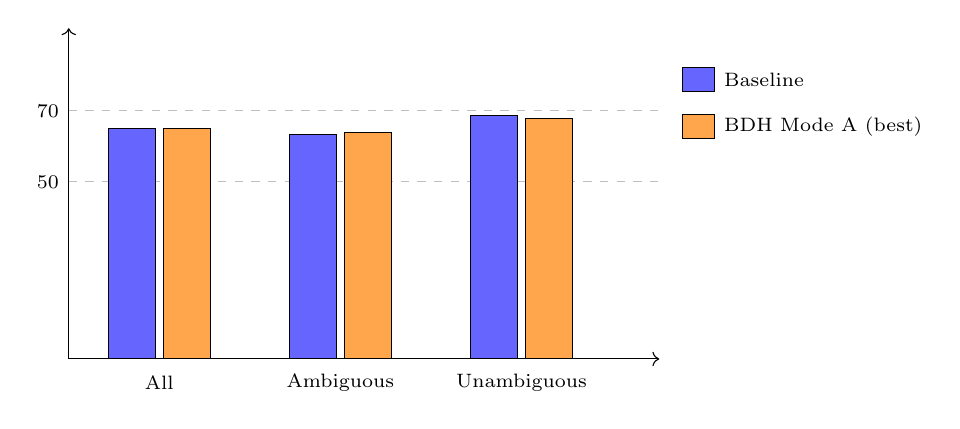
\begin{tikzpicture}[scale=1, every node/.style={font=\scriptsize}]
    \def\scaleY{0.045}
    \draw[->] (-0.5,0) -- (7,0);
    \draw[->] (-0.5,0) -- (-0.5,4.2);
    \draw[dashed, gray!50] (-0.5,{70*\scaleY}) -- (7,{70*\scaleY});
    \node[left] at (-0.5,{70*\scaleY}) {70};
    \draw[dashed, gray!50] (-0.5,{50*\scaleY}) -- (7,{50*\scaleY});
    \node[left] at (-0.5,{50*\scaleY}) {50};

    \draw[fill=blue!60] (0,0) rectangle (0.6,{64.92*\scaleY});
    \draw[fill=orange!70] (0.7,0) rectangle (1.3,{65.09*\scaleY});
    \node at (0.65,-0.3) {All};

    \draw[fill=blue!60] (2.3,0) rectangle (2.9,{63.37*\scaleY});
    \draw[fill=orange!70] (3.0,0) rectangle (3.6,{63.98*\scaleY});
    \node at (2.95,-0.3) {Ambiguous};

    \draw[fill=blue!60] (4.6,0) rectangle (5.2,{68.77*\scaleY});
    \draw[fill=orange!70] (5.3,0) rectangle (5.9,{67.87*\scaleY});
    \node at (5.25,-0.3) {Unambiguous};

    \draw[fill=blue!60] (7.3,3.4) rectangle (7.7,3.7);
    \node[right] at (7.7,3.55) {Baseline};
    \draw[fill=orange!70] (7.3,2.8) rectangle (7.7,3.1);
    \node[right] at (7.7,2.95) {BDH Mode A (best)};
  \end{tikzpicture}
  }
  \end{center}
  \footnotesize\textit{Bar chart: headline pair (baseline vs.\ winning
  Mode A). Full 3-mode sweep in the table above.}
\end{frame}

% ------------------------------------------------------------------
\begin{frame}{Interpretation}
  \begin{itemize}
    \item \textbf{Mode A} is the first (and only) formulation pointing
      in the hypothesis's predicted direction: beats baseline on
      ambiguous scenes ($+0.61$) while ceding ground on unambiguous
      ($-0.90$) — a genuine disambiguation trade-off.
    \item \textbf{Modes B and C both do worse specifically on
      ambiguous scenes} ($-1.20$ and $-5.18$ vs.\ baseline)
      \emph{despite both having} an explicit outer-product associative
      memory, same as Mode A.
  \end{itemize}
  \vspace{0.2cm}
  \begin{exampleblock}{Key insight}
    The win isn't just ``having associative memory'' — it's
    specifically Mode A's \textbf{causal text-self-contextualization}
    step (words attend to each other before regions query them). This
    directly motivates the BDH$\to$attention hybrid idea (Future Work).
  \end{exampleblock}
  \begin{alertblock}{Caveat}
    Single seed per variant — a $\sim$1 AP50 gap on 830 images carries
    meaningful noise. Encouraging, not yet conclusive.
  \end{alertblock}
\end{frame}

\section{Where We Stand vs.\ SOTA}

% ------------------------------------------------------------------
\begin{frame}{Where We Stand — Same-Class Comparison}
  \small ThinkDeeper (Liao et al., Nov 2025, ViT+BERT+world-model+hypergraph,
  \textbf{76.64} AP50) is \#1 on Talk2Car — but its own Table~1 shows a clear
  bracket structure by backbone class:
  \begin{table}
    \centering\footnotesize
    \begin{tabular}{lccl}
      \toprule
      Model & Backbone & AP50 (test) & Params \\
      \midrule
      AttnGrounder (paper) & CNN & 61.32 & 75.84M \\
      \textbf{Ours: BDH Mode A} & CNN & \textbf{65.09 (val)} & \textbf{76.63M} \\
      CMSVG & CNN (EfficientNet) & 68.61 & --- \\
      VL-BERT & CNN+BERT & 70.03 & $\sim$118M \\
      RSD-LXMERT & LXMERT & 72.64 & $\sim$210-230M \\
      ThinkDeeper & ViT+BERT+\ldots & 76.64 & not stated \\
      \bottomrule
    \end{tabular}
  \end{table}
  \begin{block}{Reframed target}
    Not ``reach 76.64'' (needs a full transformer/VLM backbone swap —
    a different project). Realistic, honest target: \textbf{beat
    CMSVG's 68.61} — top of our same-class (CNN, non-VLM) bracket.
  \end{block}
  \small We're also meaningfully smaller than the transformer-class
  models (60-70\% of VL-BERT, $\sim$1/3 of RSD-LXMERT) and trivially
  smaller than VLM-based ones (7B--72B params).
\end{frame}

\section{What's Novel Here}

% ------------------------------------------------------------------
\begin{frame}{What's Genuinely New Here}
  \footnotesize\textit{Based on our literature review — framed as ``no
  prior work found,'' not an unfalsifiable ``first ever.''}
  \vspace{0.15cm}
  \begin{alertblock}{Headline novelty 1: BDH applied to cross-modal grounding}
    \footnotesize BDH's own authors tested it on \textbf{single-modality}
    vision classification (E-BDH, image-only) and language modeling —
    never on cross-modal vision-language fusion. No evidence found of
    BDH applied to visual grounding, or to Talk2Car, anywhere in the
    literature. This is the first cross-modal grounding application.
  \end{alertblock}
  \begin{alertblock}{Headline novelty 2: three original non-causal kernel adaptations}
    \footnotesize BDH was designed causal/autoregressive (language has
    sequence order; grounding doesn't). Modes A/B/C are original
    designs adapting BDH's associative-memory mechanism to a
    non-causal, bimodal setting — not a plug-and-play reuse.
  \end{alertblock}
  \footnotesize
  \begin{itemize}\setlength{\itemsep}{2pt}
    \item \textbf{Significant — quantitative ambiguity stratification}:
      nuScenes-joined same-class-object counting on Talk2Car's own
      val split (not shipped with the dataset) — enables testing the
      hypothesis at the sub-population level, not just in aggregate.
    \item \textbf{Significant — the fusion trim as a confound control}:
      deliberately holds params near-parity ($+1\%$) with baseline, so
      the mechanism swap is the \emph{only} variable — unlike most SOTA
      papers, which change backbone + mechanism + data together, making
      it hard to attribute their gains to any one factor.
  \end{itemize}
\end{frame}

\section{Methodology}

% ------------------------------------------------------------------
\begin{frame}{A Note on Methodology: Why Val, Not Test}
  \begin{itemize}
    \item Talk2Car's test-set ground truth has \textbf{never been
      publicly released} — the only historical evaluation path was an
      AIcrowd-hosted server (ECCV 2020 C4AV challenge).
    \item That server \textbf{closed to submissions in August 2020}.
      No evidence of a live replacement.
    \item Papers reporting Talk2Car ``test'' scores since then
      (RSD-LXMERT 2022, CAVG/ThinkDeeper 2024--2025) still point to
      that same dead link — their numbers are most likely
      \textbf{self-reported, not independently verified}.
  \end{itemize}
  \vspace{0.3cm}
  \begin{alertblock}{Our choice}
    Report \textbf{val-set AP50 only}, explicitly caveated against
    other papers' self-reported test numbers. Less flattering,
    more honest — directionally informative, not strict
    apples-to-apples.
  \end{alertblock}
\end{frame}

\section{Future Scope}

% ------------------------------------------------------------------
\begin{frame}{In Progress \& Next Up}
  \begin{exampleblock}{In progress}
    \footnotesize \textbf{Tversky + Focal loss} (Salehi et al.\ 2017 /
    Lin et al.\ 2017 — ThinkDeeper's own aux-loss references)
    replacing plain BCE on the $\beta$/attention-map supervision. One
    loss swap, no architecture change — targets foreground/distractor
    imbalance, plausibly most relevant in ambiguous scenes. Training
    now on Mode A.
  \end{exampleblock}
  \footnotesize
  \begin{itemize}\setlength{\itemsep}{1pt}
    \item \textbf{BDH stacking} (2-3 layers): current module is a
      single lift$\to$read$\to$gate$\to$decode pass. Tests ``does
      more memory depth help.''
    \item \textbf{BDH$\to$attention hybrid}: motivated by today's
      insight — memory builds text context, then standard attention
      aligns.
    \item \textbf{Depth/distance prior}: reuse the 3D data already
      pulled from nuScenes (Step 6) — no new model needed.
    \item \textbf{Pretrained text encoder} (DistilBERT/MiniLM):
      replaces 2014-era GloVe+BiLSTM — contained scope, doesn't touch
      BDH, vision backbone, or detection head.
  \end{itemize}
  \footnotesize\textit{Scoped out for now: YOLOv7/YOLO26 backbone+head
  swap — legitimate lever, but a much bigger, separate engineering
  track that doesn't test the memory hypothesis.}
\end{frame}

% ------------------------------------------------------------------
\begin{frame}{Why Keep Pursuing This}
  \begin{enumerate}
    \item \textbf{We already have a real, encouraging signal.} Mode A
      shows the exact hypothesis-predicted trade-off — not just
      infrastructure readiness, an actual result worth building on.
    \item \textbf{The infrastructure cost is already paid.} Data
      pipeline, drop-in BDH module (3 modes), training loop, and the
      stratified evaluator are all built and validated end-to-end.
      Remaining work is experiment iteration, not engineering.
    \item \textbf{Low marginal model cost.} BDH adds $\sim$1\%
      parameters — stays a clean, fair test of the \emph{mechanism}.
    \item \textbf{Directly tests a live hypothesis} from recent
      literature (BDH / Dragon Hatchling, $<$1 year old) in a task
      setting the original work never evaluated.
  \end{enumerate}
\end{frame}

% ------------------------------------------------------------------
\begin{frame}{Summary}
  \begin{itemize}
    \item Built a validated, drop-in BDH swap (3 kernel modes) for
      AttnGrounder, plus a from-scratch baseline reproduction (64.92
      AP50 vs.\ paper's 63.30\%).
    \item Built a nuScenes-based pipeline to stratify Talk2Car val by
      scene ambiguity (830 ambiguous / 333 unambiguous).
    \item \textbf{Mode A wins the ablation}: beats baseline on
      ambiguous scenes specifically ($+0.61$) — the first real signal
      supporting the hypothesis. Modes B/C do not.
    \item We're competitive with the CNN-class SOTA bracket
      (61--69 AP50) at a smaller parameter count than most peers.
    \item Next: Tversky+Focal loss (running now), then BDH stacking,
      BDH$\to$attention hybrid, and a pretrained text encoder.
  \end{itemize}
  \vspace{0.4cm}
  \centering\Large Thank you --- questions welcome.
\end{frame}

\end{document}
